\label{sec:background}
In diesen Kapitel soll die Problemstellung der mangelhaften Softwaredokumentation analysiert werden. Hierzu muss zunächst der Begriff \enquote{Softwaredokumentation} definiert werden. Anschließend werden einige Statistiken präsentiert, die zeigen, dass eine mangelhafte Softwaredokumentation ein reales Problem für Entwickler ist. Des Weiteren sollen die Folgen von schlecht dokumentierten Code analysiert werden. Zudem wird in diesem Kapitel die Grundlagen von Javadocs erläutert, welches das Tool später als Grundlage für die Analyse der Dokumentation nutzt. Zuletzt werden noch einige Programme vorgestellt, die unter anderem auch die Dokumentation von Software bewerten können. 

\section{Definition der Softwaredokumentation}
Um den Begriff \enquote{Softwaredokumentation} zu definieren, sollte zunächst der Begriff \enquote{Dokumentation} definiert werden. Das IEEE  definiert diesen Begriff als jede textliche oder bildliche Information, welche Aktivitäten, Anforderungen, Abläufe oder Ergebnisse beschreibt, definiert, spezifiziert, berichtet oder zertifiziert \cite[S. 28]{IEEEStandardGlossaryofSoftwareEngineeringTerminology}. Kurz zusammengefasst beschreibt eine Dokumentation also, wie sich eine Komponente aufgebaut ist oder wie sie sich verhält.

Diese abstrakte Definition lässt sich so auf Softwareentwicklung übertragen. In \cite[S. 125]{Softwaredocumentationandstandards} wird Softwaredokumentation als eine Sammlung von technischen Informationen beschrieben, die für Menschen lesbar sind und die die Funktionen, Benutzung oder das Design eines Softwaresystems beschreiben. So beschreibt der Autor in [], dass die Hauptaufgabe beim Programmieren nicht sein sollte, einen Computer zu erklären, was er machen sollte, sondern anderen Menschen zu erklären, was der Computer machen sollte.

Im Kontext dieser Bachelorarbeit sollen allerdings nur bestimmte Arten der Softwaredokumentation betrachtet werden, da eine umfassende Betrachtung innerhalb der vorgegebenen Zeit nicht möglich ist. Die wichtigste Kategorie im Kontext der Bachelorarbeit sind bestimmte Kommentare im Quelltext eines Programms, die zu den sogenannten Inline-Kommentaren gehören. Diese Kommentare werden wie normale Kommentare erkannt und werden daher nicht Bestandteil des kompilierten Programms. Nichtsdestotrotz haben diese spezifischen Kommentare aber eine bestimmte Struktur, die eine leichte Verarbeitung durch Computerprogramme ermöglicht und gleichzeitig trotzdem für Menschen lesbar bleibt. In vielen Fällen werden diese Kommentare einer bestimmten Komponente zugeordnet, wobei dies oft dadurch geschieht, dass der Kommentar direkt vor dieser Komponente steht.

Andere Möglichkeiten zur Dokumentation, die nur hier kurz erwähnt werden sollen, sind UML-Diagramme, Handbücher und  Readme-Dateien.


\section{Statistiken zu Softwarequalität}
Dass in vielen Fällen die Softwaredokumentation vernachlässigt wird, ist durch viele Studien belegt. Eine Umfrage aus dem Jahr 2002 mit 48 Teilnehmern belegt beispielsweise, dass Anforderungs- oder Spezifikationsdokumente nur selten bei Änderungen am Quellcode angepasst werden. Außerdem verwenden viele Entwickler häufig Programme, die nicht für Dokumentationszwecke entwickelt wurden (z. B Microsoft Word etc.) \cite[S. 28-29]{TheRelevanceofSoftwareDocumentationToolsandTechnologies:ASurvey}. Diese Programme sind leicht zu bedienen und sehr flexibel, verwenden jedoch teilweise proprietäre Dateiformate und sind daher nicht unbedingt effizient.

Eine weitere Studie aus dem Jahr 2019 verdeutlicht viele Aspekte aus der vorgenannten Umfrage. Es wurden dabei Daten aus Stack Overflow, GitHub Issues und Pull Requests und Mailing-Listen automatisiert heruntergeladen und dann von den Autoren analysiert, ob und inwieweit mit mangelhafter Softwaredokumentation zu tun haben.  Die Studie liefert klare Indizien dafür, dass die Softwaredokumentation in vielen Fällen nicht komplett, nicht auf dem neuesten Stand oder sogar nicht korrekt ist. Des Weiteren ist die Softwaredokumentation nicht gut nutzbar oder schlecht lesbar, sodass der Vorteil verloren geht\cite[S.1201 -1204]{SoftwareDocumentationIssuesUnveiled}.
\section{Javadoc}
Javadoc \cite{Javadoc} ist ein Tool zur Generierung von Dokumentationen, das sich als de-facto Standard für Dokumentationen in der Programmiersprache Java etabliert hat \cite[S. 249]{JavadocViolationsandTheirEvolutioninOpen-SourceSoftware}.  Javadoc besteht aus speziellen Java-Kommentaren, die an bestimmten Stellen im Quellcode eingefügt werden und daher bei der Kompilation nicht berücksichtigt werden. Ein Javadoc-Block beschreibt immer ein bestimmtes Modul (z. B. eine Klasse, Methode oder Feld).Es beginnt mit der Zeichenkette \enquote{/**}, wobei die ersten beiden Zeichen \enquote{/*} den Beginn eines mehrzeiligen Kommentars in Java einläuten, und endet mit \enquote{*/}. Zunächst sollte am Anfang des Blocks eine generelle Zusammenfassung der Komponente geschrieben werden. Danach können sogenannte Tags, die mit dem \enquote{@}-Zeichen beginnen, benutzt werden. Diese beschreiben wiederum einen bestimmten Teilbereich einer Komponente. Es ist zudem Konvention, dass jede Zeile in einem Javdoc-Block mit einem Asterisk beginnt. Tabelle \ref{tab:table_javadoc_method} beschreibt einige Tags für Java-Methoden:
\begin{table}[h]
    \centering
    \begin{tabular}{m{4cm}|m{4cm}|m{7cm}}
    Tag & zusätzliche Parameter &Beschreibung\\
    \hline
        @param  & Paramatername & Beschreibt einen Methodenparameter\\
        \hline
         @return & & Beschreibt den Rückgabewert der Methode, sofern er existiert \\
         \hline
         @throws &Exception & Beschreibt welche Exceptions diese Methode werfen kann und möglichst unter welchen Umständen dies passiert \\
           \hline
         @deprecrated & & Falls diese Methode veraltet ist und nicht mehr verwendet werden sollte, kann hier eine Alternative beschrieben werden. \\
           \hline
         
           \hline
         
         
         
         
    \end{tabular}
    \caption{Wichtige Javadoc-Tags}
    \label{tab:table_javadoc_method}
\end{table}
Quelltext \ref{lst:simple_javadoc} zeigt ein Beispiel für eine  \enquote{gelungene} Verwendung von Javadoc. Zunächst wird der Zweck der Methode beschrieben, anschließend wird jeder Parameter erläutert. Dabei sollte in komplexeren Fällen auch erklärt werden, welche Werte gültig für den Parameter sind. Danach folgt eine Beschreibung des Rückgabewertes, welche am besten auch jeden möglichen Fall abdeckt. Mit \enquote{{@code ...}} kann auf einen Parameter referenziert werden. Mit diesen Informationen kann der Programmierer leicht überblicken, wie eine Methode genutzt werden, sodass die Einarbeitungszeit und die Fehleranfälligkeit reduziert werden kann.  
		\begin{figure}
			\lstinputlisting
			[caption={Beispielhafter Javdoc-Block für einfache Methode},
			label={lst:simple_javadoc},
			captionpos=b,language=java, basicstyle=\footnotesize, tabsize=1, showstringspaces=false,  numbers=left]
			{figures/ternary.java}
		\end{figure}

Auf der offiziellen Oracle-Webseite werden weitere empfehlenswerte Tipps für gute Javadoc-Kommentare gegeben, die hier auszugsweise und ohne besondere Reihenfolge wiedergegeben werden\cite{HowtoWriteDocCommentsfortheJavadocTool}:
\begin{itemize}
    \item Nicht in jeden Fall vollständige Sätze verwenden, aber klar formulieren, was die Aufgabe einer Komponente ist
    \item In der dritten und nicht in der zweiten Person schreiben
    \item Nicht repetitiv sein. Ein Kommentar, der im Wesentlichen nur den Namen einer Komponente wiedergibt, hat keinen Mehrwert
    \item  Beschreibungen von Methoden sollten mit einem Verb beginnen
    \item bei einem Verweis auf das aktuelle Objekt sollte das spezifische \textit{this} statt des allgemeineren \textit{the} verwendet werden
    \item Bezeichner sollten in mit \textit{<code></code>} umschlossen werden, um deutlich zu machen, dass dies eine andere Komponente ist
    \item Der Kommentar sollte eventuelle Unterschiede unter verschiedene Plattformen erläutern
    \item Die Dokumentation sollte erläutern, wie sich die Komponente in Randfällen verhält
    
\end{itemize}
Diese Javadoc-Blöcke können dann von dem gleichnamigen Tool in eine HTML-Datei umgewandelt werden und ermöglichen den Entwicklern damit einen komfortablen Überblick über alle Komponenten eines Moduls. Zudem könne Javadoc-Blöcke ebenfalls HTML-Inhalte besitzen, die dann von Javadoc in die HTML-Datei übernommen werden, sodass der Entwickler beispielsweise Tabellen zur übersichtlichen Präsentation  von Informationen verwenden kann. Abbildung \ref{fig:javadoc_example_screenshot} zeigt, wie eine Methode mittels Javadoc in HTML beschrieben wird. 
\begin{figure}[h]
    \centering
    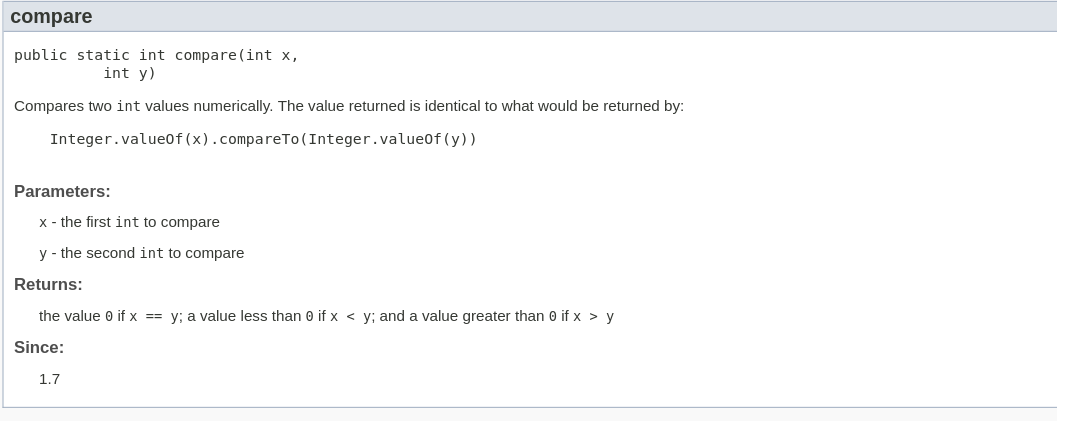
\includegraphics[width=\columnwidth]{figures/javadoc_screenshot.png}
    \caption{Gerenderte HTML-Ausgabe von javadoc}
    \label{fig:javadoc_example_screenshot}
\end{figure}

in Javadoc-Kommentar wird vererbt und muss daher für eine abgeleitete Klasse nicht neu geschrieben oder redundant geklont werden. Dies ist sinnvoll, da abgeleitete Klassen einen Vertrag erfüllen müssen, der bei einer guten Dokumentation auch schon in der Javadoc-Dokumentation beschrieben wird. Auch bei Methoden, die aufgrund einer Schnittstelle implementiert werden müssen, ist eine Neudefinition des Javadoc-Kommentar unnötig. Falls sinnvoll, kann aber dennoch ein eigener Javadoc-Kommentar erstellt werden, der allerdings den Kommentar der Quelle vollständig ersetzt. Mit \textit{@inheritDoc} kann der ursprüngliche Kommentar aber trotzdem eingefügt werden.

Für andere Programmiersprachen gibt es vergleichbare Werkzeuge, die ähnliche Funktionen anbieten und bei denen die Dokumentationen mit einer relativ ähnlichen Syntax erstellt werden. Dazu gehören beispielsweise Doxygen für C++-Programme oder der PHP-Documentor für PHP-Programme. 
\section{Tools zur Bewertung von Javadoc}
Um die Qualität der Softwaredokumentation in Javadoc zu bewerten, gibt es bereits einige Programme. In vielen Fällen handelt es sich dabei um Programme, die nicht auf die Bewertung der Softwaredokumentation beschränkt sind, sondern auch andere Fälle von unsauberem Code erkennen können. Da die Bewertung der Dokumentation nicht der primäre Zweck der Programme ist, sind die verwendeten Metriken recht allgemein und erkennen viele Problemfälle nicht. Nichtsdestotrotz sind diese Programme, dadurch dass sie viele \enquote{Code-Smells} erkennen, sehr gut geeignet, um sich ein gutes Bild über die Qualität des Quellcodes zu verschaffen und den Entwickler zu sauberer Arbeit auch außerhalb von Kommentaren zu ermuntern.
\subsubsection{Checkstyle}
Eines der bekanntesten Programme ist Checkstyle \cite{Checkstyle}. Mit Checkstyle lässt sich beispielsweise prüfen, ob alle Methoden überhaupt ein Javadoc-Block besitzen, der Javadoc-Block korrekt platziert wurde oder ein Javadoc-Tag wie zum Beispiel \enquote{@deprecated} auch mit einer zusätzlichen Begründung versehen wurde. 
\subsubsection{PMD}
Des Weiteren gibt es das Programm PMD\cite{PMD}, das ebenfalls einige Metriken für Javadoc mitliefert. Dazu gehört, ob jede öffentliche Methode dokumentiert wurde oder die Kommentare generell zu lang sind. Interessanterweise gibt es auch die Möglichkeit, bestimmte Wörter, die als anstößig empfunden werden, aus Kommentaren und Dokumentationen auszuschließen, damit Kommentare neutral bleiben. 
\subsubsection{Javadoc}
Das oben erwähnte Javadoc-Tool bietet ebenfalls die Möglichkeit, beim Generieren der HTML-Datei die Qualität des Javadocs zu prüfen. Dabei werden vor allem fehlende Tags für Parameter etc. bemängelt. Zudem erkennt Javadoc auch Tabellen mit fehlender Überschrift und andere Designmängel, die in der HTML-Seite später auffallen. Auch fehlerhaftes HTML kann erkannt werden.

\section{Theoretische Arbeiten im Bereich der Bewertung von Softwaredokumentation}

Neben den praktischen Tools, die den Softwareentwickler bei der Bewertung der Softwaredokumentation unterstützen, wurden auch einige wissenschaftliche Arbeiten veröffentlicht, die sich mit Metriken über Softwaredokumentation auseinandersetzen. 


\subsection{Quasoledo}
In \cite[S. 4-10]{HowDocumentationEvolvesoverTime} geben die Autoren einige Metriken an, die sie für die Bewertung der Softwaredokumentation als nützlich erachten. Dazu gehören:
\begin{description}
    \item[ANYJ] Anteil der dokumentierten Deklarationen an allen Deklarationen
    \item[DIR] Anteil dokumentierter Items(Methodenparameter, Rückgabewerte von Methoden und Deklarationen) an allen Items
    \item[ANYC\textsubscript{method}] Anteil der Methoden mit irgendwelchen Kommentaren als Header (z.B. reine mehrzeilige) an allen Methoden
    \item[KINCAID] Lesbarkeitsformel nach \cite[S. 50]{ThePrinciplesofReadability}
\end{description}
Die Arbeit wertet anschließend die Javadoc-Dokumentation von Eclipse aus und findet heraus, dass öffentliche Methoden häufiger dokumentiert sind und ihre Dokumentation oft lesbarer ist. Außerdem wenden die Autoren das Tool, das \textit{Quasoledo} genannt wird, auf die gesamte Versionshistorie von Eclipse bis zum 8. April 2006 an und plotten den Verlauf der Dokumentationsqualität über diesem Zeitraum. Dabei wird sichtbar, dass die Qualität am Anfang des Projektes noch sehr stark schwankt, aber nach einiger Zeit recht konstant bleibt. 
\subsubsection{JavaDocMiner}
Eine weitere Arbeit, die eine der Grundlagen dieser Bachelorarbeit ist, ist der \enquote{JavaDocMiner} \cite[S. 68-79]{AutomaticQualityAssessmentofSourceCodeComments:TheJavadocMiner}. In dieser Arbeit wird ein Programm beschrieben, welches mittels einfachen Heuristiken eine Einschätzung der Softwaredokumentation beschrieben. Das Tool extrahiert aus XML-Dateien, die mittels eines selbst geschriebene Doclet aus Javadoc erstellt wurden, die notwendigen Informationen und wendet dann auf diese XML-Struktur die Metriken an. 

Insgesamt verwendeten die Autoren die folgenden Metriken. Metriken wie \textit{ANYJ} oder \textit{DIR} wurden dabei auch verwendet, werden aber hier ausgelassen:
\begin{description}
    \item[WPJC] Durchschnittliche Anzahl an Wörtern pro Javadoc-Kommentar
    \item[ABB] Zählt die Anzahl von Abkürzungen, da diese laut der Arbeit vermieden werden soll
    \item[Fog-Index] Formel, die die Anzahl der schulischen Ausbildungsjahren angibt, um einen Text zu verstehen 
\end{description}

Anschließend wendeten die Autoren das Tool auf den Quellcode an und prüften, ob es eine Korrelation zwischen der Anzahl an Bugs und der Qualität der Dokumentation nach den benannten Metriken und fanden dabei heraus, dass die Flesch-Metrik nur wenig mit der Anzahl der Bugs korreliert, während andere Metriken wie z. B. \textit{ANYJ} eine starke negative Korrelation gab. 

\subsubsection{Doc2Spec}
Die Autoren in \cite[S. 307ff.]{InferringResourceSpecificationsfromNaturalLanguageAPIDocumentation} erläutern ein Verfahren, um herauszufinden, ob eine API korrekt verwendet wurde. Dabei werden die Javadoc-Kommentare einer API analysiert und dann mit der Verwendung der API verglichen, um Fehler bei der Handhabung der API zu finden. 

Für jede dokumentierte Methode der API wird ein Aktion-Ressource-Paar erstellt. Diese beschreibt welche Aktion auf welche Ressource ausgeführt. Bei einer Methode namens \textit{close}, die mit dem englischen Text \enquote{Initiates close of the connection handle at the
application level} dokumentiert wird, lässt sich beispielsweise schlussfolgern, dass das Aktion-Ressource-Paar \textit{(close,connection)} sein kann; denn die Aktion \textit{close} bezieht sich auf die Ressource \textit{connection}. Dabei sind aber manchmal mehrere Aktion-Ressource-Paare möglich\cite[S. 308]{InferringResourceSpecificationsfromNaturalLanguageAPIDocumentation}.

Anschließend werden die gefundenen Ressourcen anhand der Klassenhierarchie passend gruppiert. Außerdem werden die Aktionen in fünf Kategorien eingeordnet, die in der die meisten Java-Methoden passen\cite[S. 311]{InferringResourceSpecificationsfromNaturalLanguageAPIDocumentation}:
\begin{description}
    \item[Creation] Methoden, die eine Ressource/Objekt erstellen
    \item[Lock] Methoden, die eine Ressource sperren
    \item[Manipulation] Methoden, die irgendwie eine Ressource verändert oder auch nur lesen, und jede andere Aktion, die nicht in den anderen Schemata passt
    \item[Unlock] Methoden, die eine gesperrte Ressource wieder freigeben
    \item[Closure] Methoden, die eine Ressource endgültig freigeben oder schließen
\end{description}

Mit diesen generierten Informationen kann dann bei Quelltext, welches diese API verwendet, geprüft werden, ob die Methoden dieser Ressource in der richtigen Reihenfolge aufgerufen werden. Beispielsweise muss eine Ressource zuerst erzeugt und gesperrt werden, bevor irgendwelche Manipulationen angewendet werden. Außerdem kann geprüft werden, ob eine Ressource auch wieder freigegeben und geschlossen wird, sodass Speicherlecks verhindert werden. Dabei werden alle möglichen Ausführungspfade einer Methode geprüft, da eine fehlendes Freigeben von Ressourcen z.B. im Ausnahmefall ein häufiger Fehler sein kann. 

\subsubsection{iComment}
\enquote{\/\*iComment} \cite[S. 145ff.]{icomment} wurde hauptsächlich für C-Programme entwickelt, um Probleme zwischen der Dokumentation und dem Quellcode zu finden. Dabei konzentriert sich das Programm auf das Finden von Synchronisationsproblemen, die bei Programmen mit mehreren Threads auftauchen können.  Bei einem exklusiven Ausschluss besitzt eine Methode einen sogenannten Lock auf ein Objekt und nur diese Methode darf mit dem Objekt arbeiten.

Setzt nun die Dokumentation einen Lock voraus, aber der Programmierer hat keinen Lock angefordert, können sehr schnelle und subtile Bugs entstehen, die nur schwer findbar sind. 

Das Programm wurde auf dem Quellcode des Linux-Kernels und Mozilla angewandt und dabei mögliche Bugs gefunden, die später auch von den Entwicklern bestätigt wurden\cite[S. 146.]{icomment}.
\subsubsection{@tComment}
Ein anderer Ansatz, der ebenfalls mit Javadoc arbeitet, heißt \enquote{@tComment}\cite[S. 1ff.]{@tComment:TestingJavadocCommentstoDetectComment-CodeInconsistencies}. Dabei wurden die Konsistenz der Javadoc-Dokumentation mit dem tatsächlichen Programmcode verglichen. Anders als die vorherigen Ansätze, wird hier das Programm dynamisch ausgeführt. Dabei werden die verschiedenen Methoden und ihr dazugehörige Javadoc-Dokumentation analysiert und daraus mittels einfacher Heuristiken ermittelt, ob ein  Nullwert für einen Parameter eine Inkonsistenz zwischen Dokumentation und Quellcode offenbart.

Beispielsweise kann die Dokumentation einer Java-Methode beschreiben, dass ein Parameter nicht null sein darf. Daraus kann gefolgert werden, dass ein Nullwert für diesen Parameter zu einer Ausnahme führt. Wenn diese Ausnahme dann auch genauer in der Dokumentation genauer spezifiziert ist, sollte genau diese Ausnahme bei einem Nullwert geworfen werden. 

Falls Nullwerte explizit erlaubt sind, sollte die Methode sich dann stets korrekt verhalten und keine Ausnahmen werfen. 

\enquote{@tComment} kann mit diesen einfachen Regeln jede Methode ausführen und prüfen, ob sich die Methode tatsächlich verhält, wie die Dokumentation es beschreibt. Dabei verwendet das Programm einfache \ac{NLP}-Heuristiken in der englischen Sprache; zum Beispiel prüft das Programm, ob die kurz vor dem Wort \enquote{null} ein negierendes Wort wie \enquote{not} oder \enquote{never} auftaucht und klassifiziert dann den dazugehörigen Parameter als Parameter, der nie null sein darf. 


\section{GitHub Actions}
\subsection{Einführung}
Github Action \cite{GithubActions} ist eine von GitHub angebotene Plattform zur Vereinfachung des \ac{CI/CD}'s. Mithilfe von  Github Actions wird Programmcode ausgeführt, wenn ein bestimmtes Ereignis stattfindet. Dieses Ereignis kann z. B. ein Push-Ereignis sein, bei dem neuer Quellcode in das GitHub-Repository hochgeladen wird, oder eine neue Version des Programms zum Release freigegeben wird. Der Programmcode kann auf einem von GitHub vorbereiteten System ausgeführt werden; es ist aber auch möglich sein eigenes System dafür zur konfigurieren. Schlägt der Programmcode fehl, weil zum Beispiel ein Fehlercode ungleich null zurückgegeben wird oder ein anderer Systemfehler vorliegt, kann der Nutzer sich leicht über den Fehler informieren, indem auf die \enquote{Actions}-Registerkarte klickt. Dort kann der Nutzer auch sämtliche Ausgaben des Programms ansehen, die auf der Konsole ausgegeben werden. Die folgende nummerierte Liste beschreibt grob, wie Programmcode in Github Actions ausgeführt werden kann:
\begin{enumerate}
    \item Ein Ereignis tritt ein, indem beispielsweise neuer Programmcode mittels Push hochgeladen wird 
    \item Github wählt ein geeignetes System aus (z. B. eine virtuelle Maschine oder ein vom Programmierer hierfür konfiguriertes System
    \item Auf dem System wird der aktuelle Programmcode des Repositorys geklont (die Branch kann frei bestimmt werden) 
    \item Der Programmcode ausgeführt, dabei steht der Pfad zum geklonten Repository über die Umgebungsvariable \textit{\$GITHUB\_WORKSPACE} bereit
    \item Abhängig vom Erfolg der Ausführung des Programmcodes:
    \begin{enumerate}
        \item Bei einem Erfolg wird der Programmierer mittels eines grünen Häkchens informiert
        \item Bei einer Fehlermeldung wird der Programmierer mittels eines roten Kreuzes über den Fehlschlag informiert und hat auch Zugriff auf die Fehlermeldungen. Je nach Einstellung des Repositorys können bestimmte Aktivitäten dann auch gestoppt werden, damit fehlerhafter Programmcode nicht weiter verbreitet wird. 
    \end{enumerate}
\end{enumerate}

Ein Anwendungsfall von GitHub Actions sind automatisierte Tests. Bei einem Push-Ereignis kann der aktuelle Programmcode mit einer geeigneten Testbibliothek getestet werden, sodass im Falle eines fehlgeschlagenen Tests der Programmierer informiert wird und die notwendigen Änderungen veranlassen kann: 

\subsection{Wichtige Begriffe im Zusammenhang mit Github Action}
In der folgenden Auflistung werden einige wichtige Begriffe erläutert, die im Zusammenhang mit GitHub Actions verwendet werden und deren Kenntnis zum Verständnis wichtig ist. 
\begin{description}
    \item[Workflow] Ein Workflow(Ablauf) ist eine automatisierter Prozess, der verschiedene Jobs ausführt, wenn ein Ereignis eintritt. Der Worklflow wird durch eine YAML-Datei definiert
    \item[Job] Ein Job ist eine Ansammlung von sogenannten \enquote{Steps}, die man als Befehle interpretieren kann. Alle Befehle in einem Job werden auf der gleichen Maschine ausgeführt. Alle Jobs in einem Workflow werden standardmäßig parallel ausgeführt, da keine Abhängigkeit zwischen den Jobs vermutet wird.
    \item[Step] Ein Step(Schritt) ist ein Shell-Befehl oder ein Verweis auf eine andere GitHub Action, die von einem Job ausgeführt werden soll. Innerhalb eines Jobs werden die Steps in der definierten Reihenfolge ausgeführt. 
    \item[Action] Eine Action ist ein Programm, das in Workflows eingebunden werden kann und häufig vorkommende Aufgaben erledigt. Dies hat den Vorteil, dass Redundanz vermieden wird. Im offiziellen Marketplace von GitHub lassen sich zu vielen verschiedenen Aufgaben bereits Actions finden. Es können aber auch eigene Actions definiert werden, was weiter unten beschrieben wird. 
    \item[Runner] Als Runner wird das System bezeichnet, auf dem die Jobs ausgeführt werden. Dies ist standardmäßig ein Linux-Betriebssystem; es können aber auch Windows oder macOS zur Ausführung des Codes verwendet werden. Bei besonderen Anforderungen kann der Runner auch auf einem System laufen, auf dem der Programmierer selbst Zugriff hat.
\end{description}
\subsection{Erstellung eines Workflows}
Ein Workflow kann über die registerkarte \enquote{Actions} erstellt werden und wird intern in dem Verzeichnis \textit{.github/workflows} gespeichert. Abbildung \ref{lst:simple_workflow} illustriert eine typische Workflow-Datei, die standardmäßig erstellt wird. Der Code wird in Tabelle \ref{tab:descr_example_workflow} genauer erklärt.
\clearpage
\begin{table}[h!]
    \centering
    \begin{tabular}{c|m{10cm}}
        Zeile(n) &  Beschreibung \\\hline
         1 & Der Name des Workflows\\\hline
         2-6 & Hier werden die verschiedenen Ereignisse beschrieben, die den Workflow auslösen. Außerdem werden die Branches spezifiert, die auf das Ereignis überwacht werden sollenö\\\hline
         7 &  Dies erlaubt, dass ein Workflow auch manuell angestoßen wird, etwa zu Debugging-Zwecken\\\hline
         8-9 & Erstellt einen Job mit den Namen \enquote{Build}\\\hline
         10 & Bestimmt auf welchen System der Workflow läuft\\\hline
         11 & Beginn der einzelnen Steps\\\hline
         12 & Bestimmt, dass der Quellcode des Repositorys geklont wird und dessen Pfad über eine Umgebungsvariable zugängig gemacht wird\\\hline
         13-14 & Gibt hier als Beispiel \enquote{Hello World} aus\\\hline
         16-19 &Beispiel um mehrere Befehle sequentiell auszuführen\\\hline
         
    \end{tabular}
    \caption{Beispielhafter Workflow}
    \label{tab:descr_example_workflow}
\end{table}
		\begin{figure}[h!]
			\lstinputlisting
			[caption={Beispielhafter Workflow-Datei},
			label={lst:simple_workflow},
			captionpos=b, basicstyle=\footnotesize, tabsize=1, showstringspaces=false,  numbers=left]
			{figures/workflow_example.yaml}
		\end{figure}
	\clearpage
	\subsection{Ausführung von Workflows}
	Wenn ein Workflow durch ein Ereignis ausgeführt wird, lässt sich die Ausgabe des Workflows über die Registerkarte \enquote{Actions} anzeigen. Dabei erhält der Programmierer auch Informationen darüber, ob der Workflow erfolgreich war oder fehlgeschlagen ist. Abbildung \ref{fig:workflow_overview} zeigt die Übersicht der ausgeführten Workflows. Wie der Abbildung zu entnehmen ist, sieht der Programmierer den Commit, auf dem der Workflow ausgeführt wurde. Auf der rechten Seite befindet sich auch eine Angabe, wann dieser Workflow ausgeführt wurde. Zudem enthält die Übersicht die Information, wie lange der Prozess gedauert hat. 
	\begin{figure}[h]
	    \centering
	    
	    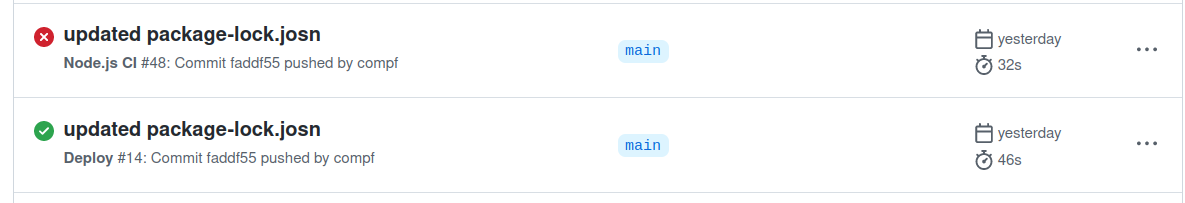
\includegraphics[width=\columnwidth]{figures/workflow_overview.png}
	    \caption{Übersicht über die ausgeführten Workflows}
	    \label{fig:workflow_overview}
	\end{figure}
	
	Durch einen Klick auf den Titel des Commits, wechselt Github auf eine weitere Seite, die grundsätzlich die gleichen Informationen wie zuvor enthält. Es ist jedoch hier möglich direkt zu der YAML-Datei zu gelangen, die diesen Workflow beschreibt. Ein weiterer Klick auf den Button mit dem Namen von dem definierten Jobs, wechselt auf eine weitere Seite, die die einzelnen Steps des Jobs auflistet und es ermöglicht, die Konsolenausgabe jedes Steps anzuzeigen. Auch eine Aufsplittung der Zeitdauer der einzelnen Steps wird angezeigt, sodass der Programmierer weiß, wie viel Zeit jeder Step benötigt. Abbildung \ref{fig:workflow_output} zeigt, wie eine solche Ausgabe auf der Konsole aussieht:
	\begin{figure}[h]
	    \centering
	    
	    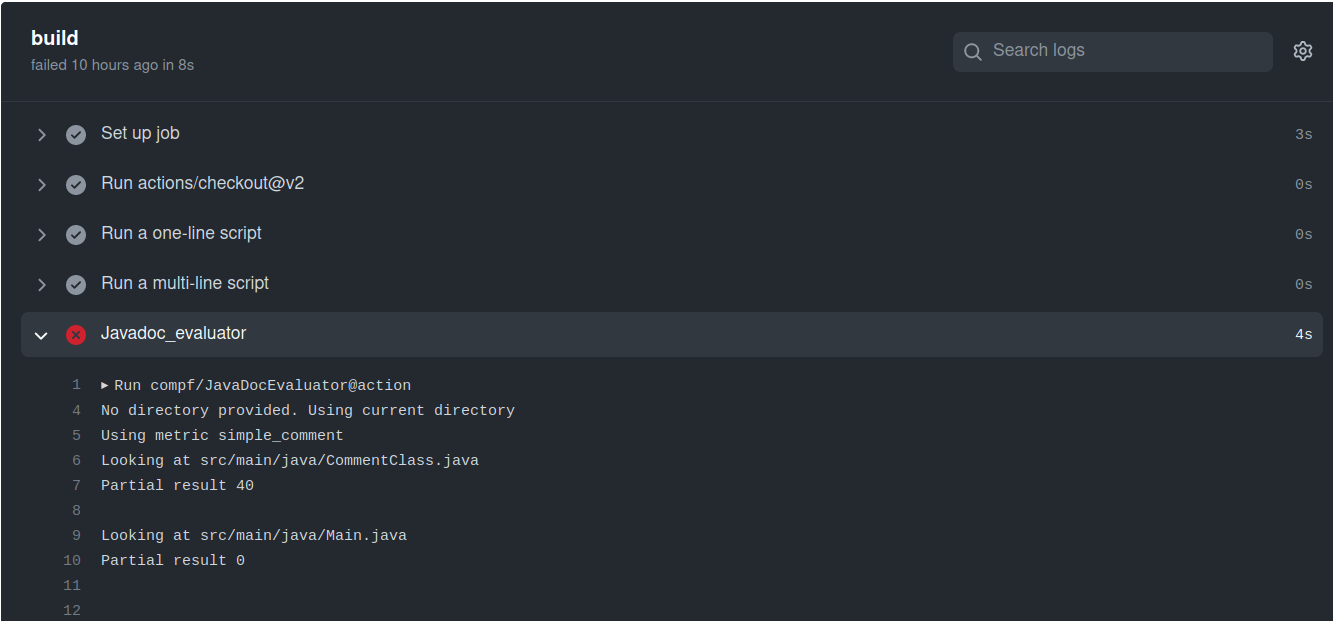
\includegraphics[width=\columnwidth]{figures/workflow_output.png}
	    \caption{Übersicht über die ausgeführten Workflows}
	    \label{fig:workflow_output}
	\end{figure}
\subsection{Erstellung einer eigenen Action}
Um eine eigene Github Action zu erstellen, muss in dem Hautpverzeichnis des Repositorys, in dem der Programmcode der Action liegt, eine Datei namens \enquote{action.yaml} oder \enquote{action.yml} erstellt werden. Abbildung \ref{lst:create_action_example} zeigt eine beispielshafte \enquote{action.yaml}
	\begin{figure}[h!]
			\lstinputlisting
			[caption={Beispielhafte Action-Konfigurationsdatei},
			label={lst:create_action_example},
			captionpos=b, basicstyle=\footnotesize, tabsize=1, showstringspaces=false,  numbers=left]
			{figures/create_action_example.yaml}
		\end{figure}
Zunächst wird der Name der Action und eine Beschreibung definiert. Anschließend können Eingabeparameter definiert werden, die später im Programm verwendet werden können. Zu jedem Parameter kann auch festgelegt werden, ob er zwingend erforderlich ist und den Standardwert des Parameters. Außerdem können Ausgabeparameter festgelegt werden, die spätere Actions als Eingabe nutzen können. Danach wird festgelegt, wie diese Action ausgeführt wird. Eine Action kann in einer JavaScript-Umgebung, in einem einem Docker-Container, oder als Liste von verschiedenen Steps ausgeführt werden. Dies wird in den folgenden Unterabschnitten kurz beschrieben.
\subsubsection{Docker-Umgebung}
In einer Docker-Umgebung kann die Action ausgeführt werden, ohne dass der Nutzer der Action sich darüber Gedanken machen muss, welche Abhängigkeiten oder Voraussetzungen diese Action benötigt. Dies ermöglicht eine fehlertolerante Ausführung des Programmscodes. Das System kann dabei sehr frei konfiguriert werden. Allerdings laufen Actions in einer Docker-Umgebung langsamer als in einer JavaScript-Umgebung. Außerdem kann zurzeit ein Action in einer Docker-Umgebung nur mittels eines Runners in Linux ausgeführt werden.

\subsubsection{JavaScript-Umgebung}
Da viele GitHub Actions in JavaScript programmiert werden, ist diese Umgebung als Option vorhanden. Es kann direkt eine geeignete Node-Umgebung installiert werden und eine JavaScript-Datei mittels \textit{main} ausgeführt werden. 

\subsubsection{Composite-Action}
Eine sogenannte Composite-Action ermöglicht es mehrere Actions in eine Action zu vereinen und so wieder Code-Redundanz zu vermeiden. Die Syntax ist dabei ähnlich wie ein normaler Workflow. 
